\documentclass[twocolumn]{article}

\usepackage{graphicx}
\usepackage{amsmath}
\usepackage{amsthm}
\usepackage{amssymb}
\usepackage{url}
\usepackage{multirow}
\usepackage{times}
\usepackage{fullpage}

\newcommand{\comment}[1]{}

\title{CS771: Group 1 \\
Online Recommender System}
\author{
\begin{tabular}{ccc}
	Akshay Kumar & Arpit Jain & Dhananjay Sharma \\
	\url{kakshay@iitk.ac.in} & \url{arpitj@iitk.ac.in} & \url{djsharma@iitk.ac.in} \\
	Dept. of CSE & Dept. of CSE & Dept. of CSE \\
	\multicolumn{3}{c}{Indian Institute of Technology, Kanpur}
\end{tabular}
}
\date{Project Report \\	% replace by ``initial'' or ``final'' as appropriate
\today}	% replace by actual date of submission or \today

\begin{document}

\maketitle

\begin{abstract}
	%
%	Abstract of the project.
	%
Online Recommender System are ubiquitous in present world. It is used by a wide array of companies like Netflix, Amazon, etc. to suggest products to their users. In this project, we have tried to build a recommender system which predicts the rating which can be given by a user. We started off with implementing already existing algorithms and then improvised it a bit and analyzed the accracies offered by each of the algorithm.
\end{abstract}

\section*{Description of Problem Statement}
As already stated, the main problem is to predict the rating given by a user to a movie. The \texttt{MovieLens} database consists of $100000$ ratings given by different users. A total of $1682$ movies have been rated by $943$ users. Each user has rated at least $20$ movies. Additionally, we are also provided with different attributes of movies and users. Specifically speaking, for a movie, we are provided with its title, different genres a movie falls, its release date, video release data and IMDB URL. For a user, we are provided with his/her demographics information such as their age, gender, occupation and zip code. Finally each user has rates some movies (atleast $20$) and we are provided the rating and the timestamp.

\section*{Approach}
The most naive approach is to pose it as a classification problem. Classification can be in any of the classes from $1$ to $5$ if a movie has been rated by the user. If we have a \emph{.arff} file with different feature vector for each rating, then this problem can be posed as a classification problem. For any rating, their exists a corresponding movie and user. So what we did was to replace movie and users by their respective attribute and classify. The whole data was split into $80 \%$ training data and $20 \%$ test data.  The results are discussed in the subsequent section.

\section*{Existing Algorithm}
There are primarily two approaches followed in movie recommender systems:
\begin{enumerate}
\item Collaborative Filtering
\item Content Based Filtering
\end{enumerate}
Content Based Filtering predicts movie rating by a user based on his previous ratings. It actually doesn't lay any accord on the connections between a user. Hence, it is efficient to predict ratings for a new user. Hence, companies adopting Content Based Ratings generally ask to new users to fill a form to know their tastes. On the the other hand, Collaborative Filtering predicts a rating based on the simillarity between two users. Similar users are goins to rate movies similarly.

\subsection*{Mathematics of the two algorithm}
The algorithms implemented by us are the ones described by Andrew Ng in Machine Learning course on Coursera.\\
\newline
Coming to the notations used,\\
\newline
$$u : \text{Set of users}\quad|u|=n_u$$
$$m : \text{Set of movies}\quad|m|=n_m$$
$$
r(i,j) = 
  \begin{cases}
    1 & \text{if user $j$ has rated movie $i$}\\
    0 & \text{otherwise}
  \end{cases}
$$
$$y(i,j)=\text{rating}\quad \text{if} \quad r_{(i,j)}=1$$
Consider the following example,\\
\newline
\begin{tabular}{| p{2cm} | p{1cm} | p{1cm} | p{1cm} | p{1cm}|}
\hline
Movie & Alice(1) & Bob(2) & Carol(3) & Dave(4)\\\hline
Love at last & 5 & 5 & 0 & 0\\\hline
Romance forever & 5 & ? & ? & 0\\\hline
Cute puppies of love & ? & 4 & 0 & ?\\\hline
Nonstop car chases & 0 & 0 & 5 & 4\\\hline
Swords vs. karate & 0 & 0 & 5 & ?\\\hline
\end{tabular}
\newline
\newline
Suppose the genre of each movie is also given (a valid assumption as it's already been provided in the movielens database). Let it be as follows:
\begin{center}
\begin{tabular}{| c | c | c |}
\hline
Movie & $x_1$(romance) & $x_2$(action)\\\hline
Love at last & 0.9 & 0\\\hline
Romance forever & 1.0 & 0.01\\\hline
Cute puppies of love & 0.99 & 0\\\hline
Nonstop car chases & 0.1 & 1.0\\\hline
Swords vs. karate & 0 & 0.9\\\hline
\end{tabular}
\end{center}
We also define the following parameters denoting the attributes of users and movies.
Corresponding to each user $j$, we define a parameter $\theta^{(j)}$. Similarly, define a parameter $x^{(i)}$ for each movie $i$.
$$\theta^{(j)} = \text{parameter vector for user $j$}$$
$$x^{(i)} = \text{parameter vector for movie $i$}$$
For user $j$, movie $i$, predicted rating would then be $(\theta^{(j)})^Tx^{(i)}$.\\
\newline
The error function for any predicted rating is $\Big((\theta^{(j)})^T(x^{(i)})-y^{(i,j)}\Big)^2$. Hence the objective funcion to be minimized is:
$$\min_{\theta^{(j)}} \frac{1}{2m^{(j)}}\displaystyle\sum\limits_{i:r(i,j)=1} \Big((\theta^{(j)})^T(x^{(i)})-y^{(i,j)}\Big)^2$$ $$+ \frac{\lambda}{2m^{(j)}}\displaystyle\sum\limits_{k=1}^{n} \Big(\theta_k^{(j)}\Big)^2$$
The last term is the penalty term for high value coefficients. Half is added for simplicity.
To learn $\theta^{(1)},\theta^{(2)},\cdots,\theta^{(n_u)}$:
$$\min_{\theta^{(1)},\theta^{(2)},\cdots,\theta^{(n_u)}} \frac{1}{2}\displaystyle\sum\limits_{j=1}^{n_u} \displaystyle\sum\limits_{i:r(i,j)=1} \Big((\theta^{(j)})^T(x^{(i)})-y^{(i,j)}\Big)^2$$ $$+ \frac{\lambda}{2}\displaystyle\sum\limits_{j=1}^{n_u} \displaystyle\sum\limits_{k=1}^{n} \Big(\theta_k^{(j)}\Big)^2$$
This can be done by using Gradient Descent Algorithm:
$$\theta_k^{(j)} := \theta_k^{(j)} - \alpha\displaystyle\sum\limits_{i:r(i,j)=1} \Big((\theta^{(j)})^T(x^{(i)})-y^{(i,j)}\Big)x_k^{(i)} \ (k=0)$$
$$\theta_k^{(j)} := \theta_k^{(j)} - \alpha\displaystyle\sum\limits_{i:r(i,j)=1} \Big((\theta^{(j)})^T(x^{(i)})-y^{(i,j)}\Big)x_k^{(i)} + \lambda\theta_k^{(j)}$$ $$(k\neq0)$$
$\alpha$ is the learning rate. The results are discussed in the results section.\\
\newline
Suppose instead of genre of different movies, we are provided with tastes of different users.\\
$$\theta^{(1)}=\begin{bmatrix} 0\\ 5\\ 0 \end{bmatrix}; \theta^{(2)}=\begin{bmatrix} 0\\ 5\\ 0 \end{bmatrix}; \theta^{(3)}=\begin{bmatrix} 0\\ 0\\ 5 \end{bmatrix}; \theta^{(4)}=\begin{bmatrix} 0\\ 0\\ 5 \end{bmatrix};$$
Here, given $\theta^{(1)},\theta^{(2)},\cdots,\theta^{(n_u)}$, we need to learn $x^{(i)}$:
$$\min_{x^{(i)}} \displaystyle\sum\limits_{j:r(i,j)=1} \Big((\theta^{(j)})^T(x^{(i)})-y^{(i,j)}\Big)^2 + \frac{\lambda}{2m^{(j)}}\displaystyle\sum\limits_{k=1}^{n} \Big(x_k^{(j)}\Big)^2$$
Summing it overall all $x^{(1)},x^{(2)},\cdots,x^{(n_m)}$, the objective function becomes:
$$\min_{x^{(1)},x^{(2)},\cdots,x^{(n_m)}} \frac{1}{2}\displaystyle\sum\limits_{i=1}^{n_m} \displaystyle\sum\limits_{j:r(i,j)=1} \Big((\theta^{(j)})^T(x^{(i)})-y^{(i,j)}\Big)^2$$ $$+ \frac{\lambda}{2}\displaystyle\sum\limits_{i=1}^{n_m} \displaystyle\sum\limits_{k=1}^{n} \Big(x_k^{(i)}\Big)^2$$
We tested Content Based Filtering on \texttt{movielens} database the results of which are discussed in the results section. Since users have very few attributes known a proiri, the second objective function was not minimized

\section*{Low Rank Matrix Factorization}
The discussion is continued from the previous section.\\
\newline
Note that we now have two different problems. Their overall structure is as follows:
\begin{enumerate}
\item Given $x^{(1)},x^{(2)},\cdots,x^{(n_m)}$, predict $\theta^{(1)},\theta^{(2)},\cdots,\theta^{(n_u)}$
\item Given $\theta^{(1)},\theta^{(2)},\cdots,\theta^{(n_u)}$, predict $x^{(1)},x^{(2)},\cdots,x^{(n_m)}$
\end{enumerate}
So, one plausible approach can be to find both $\theta$'s and $x$'s simultaneously. Start off with some random $\theta$ and update $x$ to miniimze the error. Based on this $x$, update $\theta$ to minimize error and keep doing so.
$$\theta \rightarrow x \rightarrow \theta \rightarrow x \rightarrow \theta \rightarrow x \rightarrow \theta \rightarrow x \rightarrow \theta \rightarrow x \cdots$$
Another approach is to change the objective function to find both $\theta$'s and $x$'s. The updated objective function is:
$$J(x^{(1)},x^{(2)},\cdots,x^{(n_m)},\theta^{(1)},\theta^{(2)},\cdots,\theta^{(n_u)})=$$
$$\frac{1}{2}\displaystyle\sum\limits_{(i,j):r(i,j)=1} \Big((\theta^{(j)})^Tx^{(i)}-y^{(i,j)}\Big)^2 +$$ 
$$\frac{\lambda}{2}\displaystyle\sum\limits_{i=1}^{n_m} \displaystyle\sum\limits_{k=1}^{n} \Big(x_k^{(i)}\Big)^2+\frac{\lambda}{2}\displaystyle\sum\limits_{j=1}^{n_u} \displaystyle\sum\limits_{k=1}^{n} \Big(\theta_k^{(j)}\Big)^2$$
The last two terms are simple the penalties of the two objective functions. The first term is formed by coalescing the first term of the wo objective function thereby removing the restriction of $i$ or $j$.\\
\newline
We need to minimize $J$ \emph{i.e}
$$\min_{\substack{x^{(1)},x^{(2)},\cdots,x^{(n_m)}\\ \theta^{(1)},\theta^{(2)},\cdots,\theta^{(n_u)}}} J(x^{(1)},\cdots,x^{(n_m)},\theta^{(1)},\cdots,\theta^{(n_u)})$$
One way to do it is via Gradient Descent Algorithm. Update $\theta$ and $x$ simultaneously.
$$x_k^{(i)} := x_k^{(i)} - \alpha\Big(\displaystyle\sum\limits_{j:r(i,j)=1}((\theta^{(j)})^Tx^{(i)}-y^{(i,j)})\theta_k^{(j)}+\lambda x_k^{(i)}\Big)$$
$$\theta_k^{(j)} := \theta_k^{(j)} - \alpha\Big(\displaystyle\sum\limits_{j:r(i,j)=1}((\theta^{(j)})^Tx^{(i)}-y^{(i,j)})x_k^{(i)}+\lambda \theta_k^{(j)}\Big)$$
where $\alpha$ is the learning rate.\\
\newline
This is a novel algorithm yet mysteriously simple algorithm used used in Movie Recommendation Engines. It was first demonstrated in nexflix challenge that matrix factorization models are superior of classical nearest-neighbour technoques. This methods allows incorporation of additional information such as feedback, temporal effects and confidence levels.\\
\newline
We will now try to express the same algorithm in a slightly different way. Given a set of users and a set of movies, the partial information about the ratings can be stored in a matrix whose $(i,j)^{th}$ entry corresponds to the rating of $i^{th}$ movie by $j^{th}$ user. Matrix Factorization exploits the fact that there should be some latent features that determine how a user rates an item.\\
\newline
With a set $U$ of users and $D$ of items, let $R : U,D \rightarrow U\times D$ be the rating matrix. Our task is to find two matrices $P (K \times |U|)$ and $Q(K \times |D|)$ such that their product approximates $R$.
$$R\approx P^T \times Q = \hat{R}$$
Here $K$ is the number of features chosen. Note that this is exactly the same as what we have already analyzed except for the fact that vectors have now been embedded into a matrix.\\
\newline
The rating corresponding to $u_i$ and $d_j$ would be:
$$\hat{r_{ij}}=p_i^Tq_j=\displaystyle\sum\limits_{k=1}^kp_{ik}q_{kj}$$
The error term defined here is:
$$e_{ij}^2=(r_{ij}-\hat{r_{ij}})^2=(r_{ij}-\displaystyle\sum\limits_{k=1}^kp_{ik}q_{kj})^2$$
The total error would then be,
$$E=\displaystyle\sum\limits_{(i,j)\in \kappa}e_{ij}^2=\displaystyle\sum\limits_{(i,j)\in \kappa}(r_{ij}-\hat{r_{ij}})^2$$ $$=\displaystyle\sum\limits_{(i,j)\in \kappa}(r_{ij}-p_i^Tq_j)^2+\lambda(\|p_i\|^2+\|q_j\|^2)$$
where $\kappa$ is the set of pairs of movies and users which have been rated.
Minimizing the error, the gradient descent update rule will then be:
$$p_{i} \leftarrow p_{i}+\alpha (e_{ij}q_{j}-\lambda p_i)$$
$$q_{j}\leftarrow q_{j}+\alpha (e_{ij}p_{i}-\lambda q_j)$$
The process can be stopped when the total error $E$ becomes less than a certain threshold.
\section*{Results}
We firstly experimented using a Simple classifier. The graph here shows the results obtained:
\begin{figure}
\centering
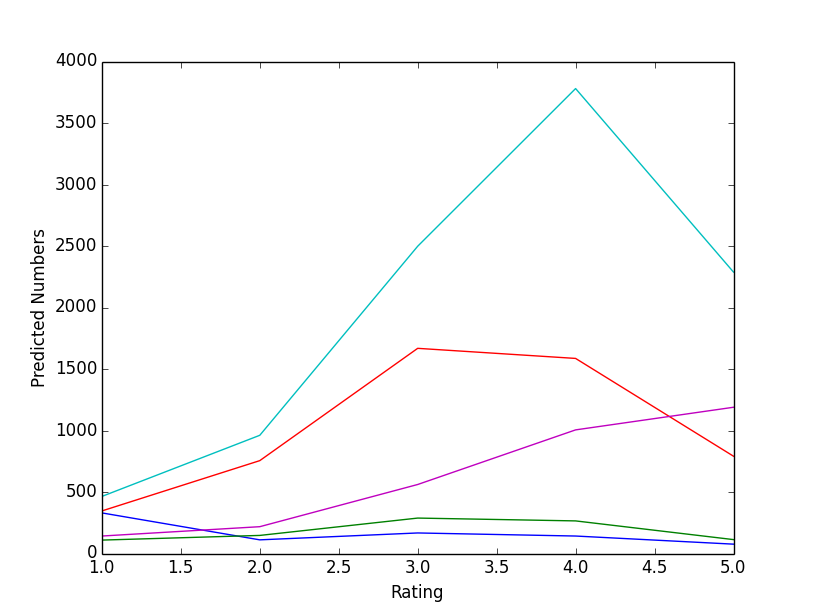
\includegraphics[width=0.5\textwidth]{figure_1.png}
\caption{A graph showing th number of predicted classes for different ratings for a simple \textbf{classifier}. The lines corresponding to ratings of $1,2,3,4,5$ are, respectively, dark blue, green, red, light blue and pink. The test dataset consisted of a total of $20000$ data points. The number of points in classes $1,2,3,4,5$ were $1391, 2192, 5182, 6778, 4457$ respectively.}
\label{fig:classifier}
\end{figure}
As evident from the figure ~\ref{fig:classifier}, the number of predicted ratings peak at the point of actual rating. For example, blue line having an actual rating of 4 peaks at the rating of 4. Similarly, pink line of actual rating 5 peaks at 5 and so on. Actually, most of the data point was concentrated around a region of actual rating plus or minus one.\\
\newline
The number of correctly classified instance for this classifier was very low \emph{viz.} $35.57 \%$. One prime reason was the fact that a classifier assumes it to be a classification problem whereas it actually is a rating prediction problem. Hence, nearly correct predicted ratings were deemed incorrect in this model.\\
\newline
Coming to the Content Based Filtering and Low Rank Matrix Factorization, the results were fairly accurate. The plotted histograms show the number of predicted users for different actual ratings \emph{viz.} $1,2,3,4,5$. As shown in the histogram, the predicted rating peaks at the actual rating most of the time. The error in this phase was only very low. We reported an error of approximately $18.11 \%$ \emph{i.e.} an accuracy of more than $81 \%$ in this method.\\
\newline
The error was calculated as follows :$-$ the Content Filtering Based Linear Regression model predicts a rating which is a real number, say $\hat{r}$. Suppose the actual rating is $r$. Then the error defined for this prediction is simpy $|r-\hat{r}|$. This is summed up over all the test instances and then the average value of this error is taken. It turned out to be nearly $18.11 \%$ which means on an average, the predicted value deviates by $18.11 \%$ from the actual value.
\begin{figure}
\centering
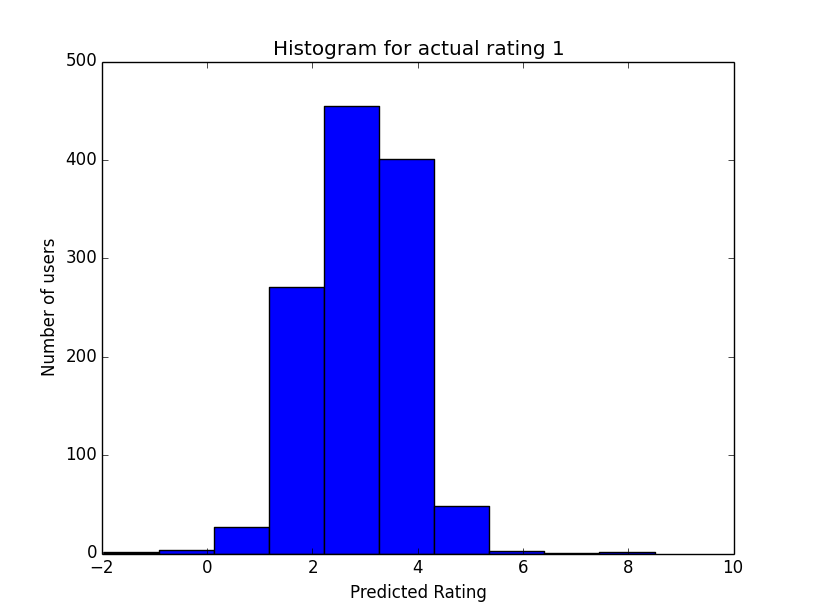
\includegraphics[width=0.4\textwidth]{hist_1.png}
\caption{Histogram for actual rating 1}
\end{figure}
\begin{figure}
\centering
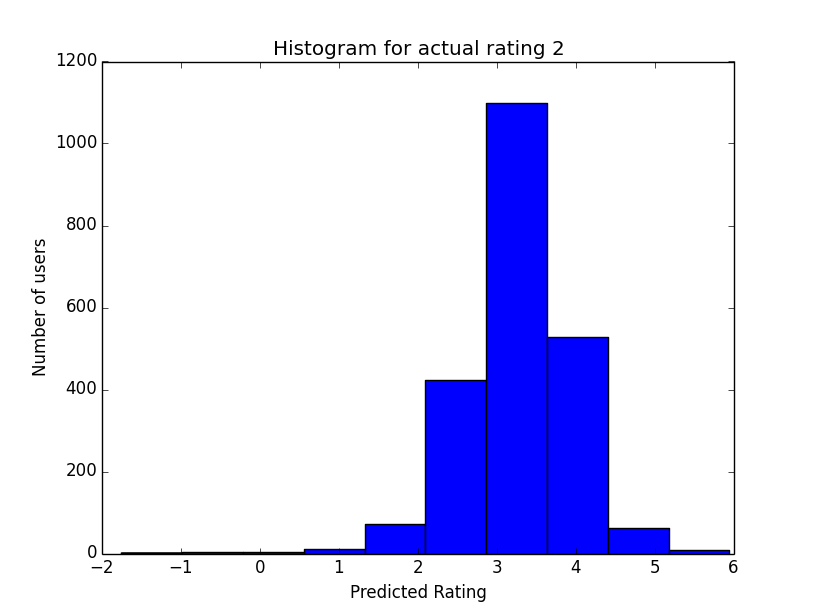
\includegraphics[width=0.4\textwidth]{hist_2.png}
\caption{Histogram for actual rating 2}
\end{figure}
\begin{figure}
\centering
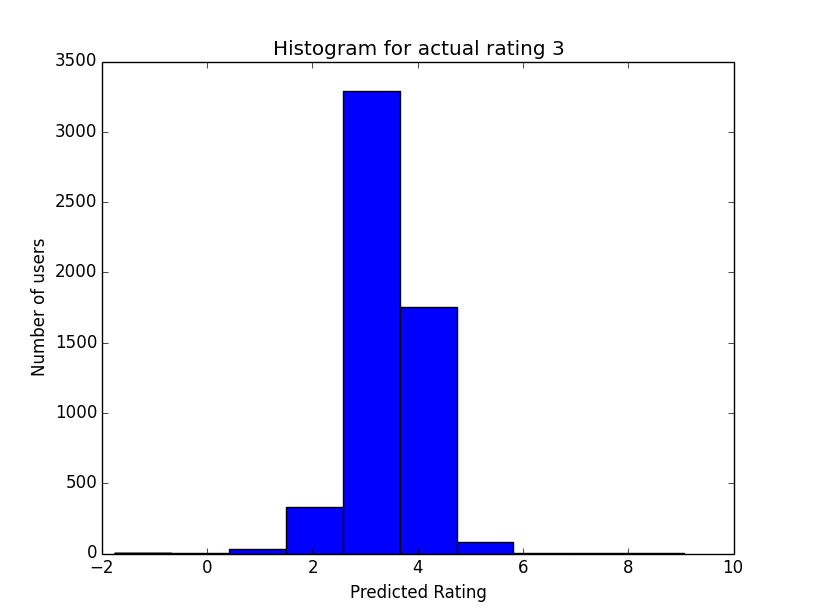
\includegraphics[width=0.4\textwidth]{hist_3.png}
\caption{Histogram for actual rating 3}
\end{figure}
\begin{figure}
\centering
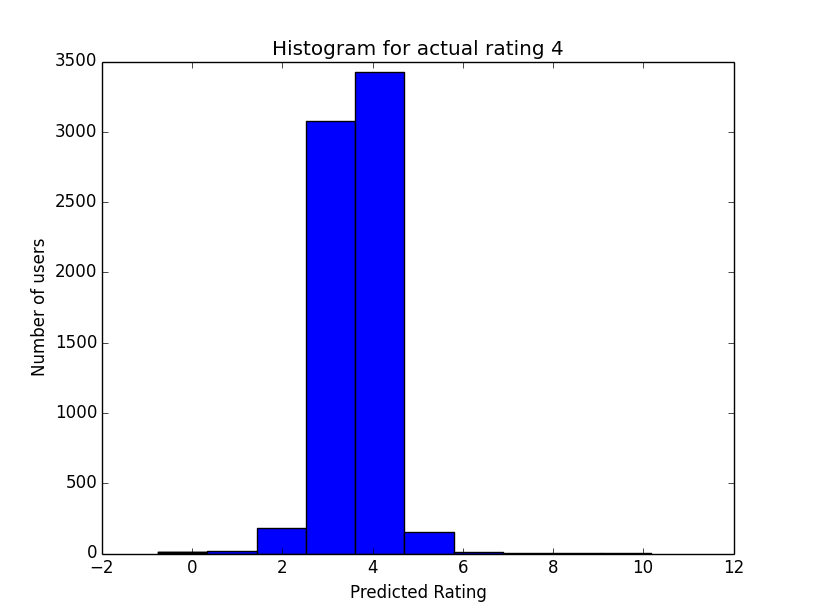
\includegraphics[width=0.4\textwidth]{hist_4.png}
\caption{Histogram for actual rating 4}
\end{figure}
\begin{figure}
\centering
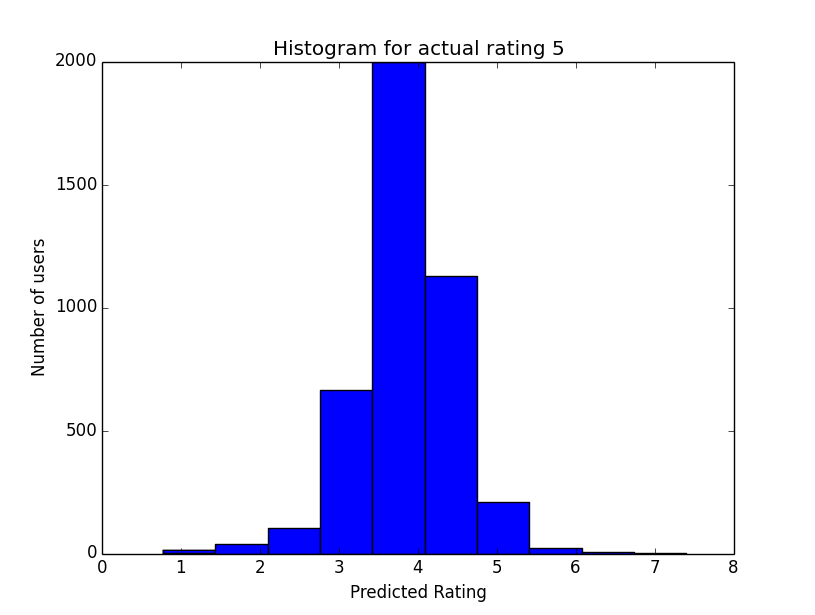
\includegraphics[width=0.4\textwidth]{hist_5.png}
\caption{Histogram for actual rating 5}
\end{figure}\\
\newline
This method lacked one major feature : inability to predict the ratings for new users because it doesn't lay any accord on user-user interaction or the similarity between two users. To mitigate this problem, we moved on to the method of Low Rank Matrix Factorization. Note that by using this method, the accuracy is not improved consideraly but now we are able to predict ratings for a entirely new user.\\
\newline
The results for this method have been omitted due to $2$ reasons:
\begin{enumerate}
\item This method didn't give considerable edge over accuracy. For exisiting users who have already rated some of the movies, the results obtained were more or less similar to the ones obtained in Content Based Filtering.
\item Training the classifier took a considerably large amount of time. Once trained, we saved this classifier as an object. Hence, we were not able to train to multiple times varying different parameters so as to obtain the best possible result.
\end{enumerate}
\section*{Shortcomings and Future Work}
Here are a few points that can be looked into:
\begin{itemize}
\item Value of $K$ for feature matrix. In the Low Rank Matrix Factorization method, this $K$ is chosen arbitrarily. This has to be fixed somehow so as to reflect different attributes/features of movies and users.
\item Prone to extreme ratings. Users with similar tastes can rate movies differently (one may be lenient whereas the other is strict). So our, our method doesn't account for this. Actually, a bias term $\mu$ can be introduced to keep a tab on this.
\end{itemize}
\section*{Platform Used}
For almost all the Meachine Learning aspect of the project, we used \texttt{weka} barring one part where we used python for building a feature matrix. We used python for building all the relavant \emph{.arff} files. For making different graphs and histograms, we again used python.
\section*{References}
\begin{enumerate}
\item Video Lecture on Mideo Recommender Systems in Machine Learning Course on Coursera by Andrew Ng
\item Matrix Factorization Techniques For Recommender Systems, \emph{Yehuda Koren, Robert Bell, Chris Volinsky}
\item Algorithms and Methods in Recommender Systems, \emph{Daniar Asanov}
\end{enumerate}
\end{document}
